% 2011 年北京卷文科第 17 题：四面体 PABC 与四条棱的中点。
% 来源 PDF：普通高考/2011/2011北京文.pdf，SHA-256 1ba0def5e75e0a4d7cc4e4e52a11a65ad598b98bc2a8e6c98df8f29fb6b9f4a6。
% 原页：第 1 页（A3 三栏）第 3 栏下部，书页码 649。
% 重绘依据：照原页拓扑——P 在上，A 在左，B 在右，C 在前下方；D、G 分别是 PA、PB 的中点，
%   E、F 分别是 AC、BC 的中点（坐标按顶点坐标取中点写入，与源图一致）。
%   实线 PA、PB、PC、AC、BC、DE、GF；虚线为隐藏棱 AB 与棱内两条线段 DG、EF。不按比例。
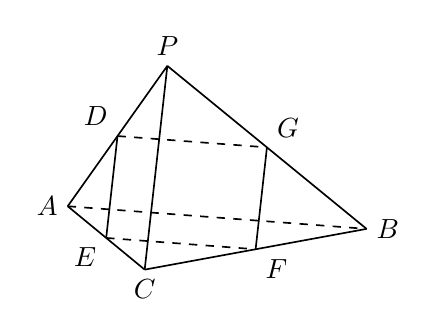
\begin{tikzpicture}[>=stealth, semithick, scale=1.15]
  % 顶点
  \coordinate (A) at (0,0);
  \coordinate (B) at (3.30,-0.25);
  \coordinate (C) at (0.85,-0.70);
  \coordinate (P) at (1.10,1.55);
  % 棱的中点：D=(P+A)/2，G=(P+B)/2，E=(A+C)/2，F=(C+B)/2
  \coordinate (D) at (0.55,0.775);
  \coordinate (G) at (2.20,0.65);
  \coordinate (E) at (0.425,-0.35);
  \coordinate (F) at (2.075,-0.475);

  % 实线
  \draw (P) -- (A);
  \draw (P) -- (B);
  \draw (P) -- (C);
  \draw (A) -- (C);
  \draw (C) -- (B);
  \draw (D) -- (E);
  \draw (G) -- (F);

  % 虚线（隐藏棱与棱内线段）
  \draw[dashed] (A) -- (B);
  \draw[dashed] (D) -- (G);
  \draw[dashed] (E) -- (F);

  \node[above] at (P) {$P$};
  \node[left] at (A) {$A$};
  \node[right] at (B) {$B$};
  \node[below] at (C) {$C$};
  \node[above left] at (D) {$D$};
  \node[above right] at (G) {$G$};
  \node[below left] at (E) {$E$};
  \node[below right] at (F) {$F$};
\end{tikzpicture}
